\documentclass[11pt,a4paper]{article}
\usepackage[a4paper,margin=0.62in]{geometry}
\usepackage[T1]{fontenc}
\usepackage[utf8]{inputenc}
\usepackage{fix-cm}
\usepackage{newtxtext}
\usepackage{amsmath,amssymb}
\usepackage{graphicx,booktabs,tabularx,array}
\usepackage{xcolor}
\usepackage{microtype}
\usepackage{setspace}
\usepackage{enumitem}
\usepackage[most]{tcolorbox}
\usepackage{tikz}
\usetikzlibrary{arrows.meta,positioning,fit,calc,shapes.geometric}
\usepackage[colorlinks=true,linkcolor=blue,urlcolor=blue]{hyperref}
\setstretch{1.01}
\setlength{\parindent}{0pt}
\setlength{\parskip}{0.18em}
\setlist[itemize]{leftmargin=1.25em,itemsep=0.02em,topsep=0.04em,parsep=0pt}

\definecolor{NTUblue}{HTML}{102A72}
\definecolor{NTUtopblue}{HTML}{074594}
\definecolor{NTUred}{HTML}{E31837}
\definecolor{MethodBlue}{HTML}{174A73}
\definecolor{Teal}{HTML}{147D85}
\definecolor{SoftBlue}{HTML}{EEF4FB}
\definecolor{SoftTeal}{HTML}{EDF7F6}
\definecolor{SoftGray}{HTML}{F5F6F8}
\definecolor{MidGray}{HTML}{DDE2E8}
\definecolor{DarkGray}{HTML}{3B4148}
\definecolor{Purple}{HTML}{6B4C9A}

\newcommand{\method}[1]{{\sffamily\bfseries\color{MethodBlue}#1}}
\newcommand{\XDB}{\method{XDomainBench}}
\newcommand{\SubspacePath}{\method{SubspacePath Pruner}}
\newcommand{\CoCurve}{\method{CoCurve}}
\newcommand{\AnchorPath}{\method{AnchorPath}}
\newcommand{\CoAx}{\method{CoAx}}
\newcommand{\SoT}{\method{SoT}}
\newcommand{\LoTR}{\method{LoTR}}
\newcommand{\worktag}[1]{\kern0.12em\textcolor{NTUred}{\textsf{\bfseries\scriptsize[#1]}}}

\newtcolorbox{thesisbox}{enhanced,colback=SoftBlue,colframe=NTUblue,boxrule=0.55pt,arc=1.2pt,left=6pt,right=6pt,top=3pt,bottom=3pt,before skip=2pt,after skip=2pt}
\newtcolorbox{smallbox}[1][]{enhanced,colback=SoftGray,colframe=DarkGray!35,boxrule=0.4pt,arc=1.2pt,left=6pt,right=6pt,top=3pt,bottom=3pt,before skip=2pt,after skip=2pt,title={#1},fonttitle=\bfseries\sffamily\small\color{NTUblue}}

\pagestyle{empty}
\begin{document}

\begin{minipage}[c]{0.78\textwidth}
{\Large\bfseries\color{NTUblue} Executive Summary of PhD QE Report}\\[-1mm]
{\large\bfseries Towards Efficient, Scalable, and Reliable Foundation Model Deployment}\\[-0.5mm]
{\normalsize\sffamily\color{DarkGray} Adaptive Model Execution and Reasoning}\\[-0.3mm]
{\normalsize Zhiren Gong \;|\; Interdisciplinary Graduate Programme, NTU}
\end{minipage}\hfill
\begin{minipage}[c]{0.18\textwidth}
\raggedleft
\includegraphics[width=\linewidth]{figures/ntu_logo.png}
\end{minipage}
\vspace{0.6mm}\hrule\vspace{1.2mm}

Foundation models now provide strong language, code, scientific, and multimodal capabilities, but deployment places that capability under heterogeneous and interactive conditions. Three constraints repeatedly matter: \textbf{(1) heavy model backbones} make full execution costly and per-scenario retraining difficult to scale; \textbf{(2) heterogeneous test-time demand} means different problems and reasoning stages need different evidence and effort; and \textbf{(3) complex internal mechanisms} create both opportunity and risk because redundancy, coupling, compensation, and self-repair shape how computation is actually carried.

\begin{center}
\resizebox{0.53\textwidth}{!}{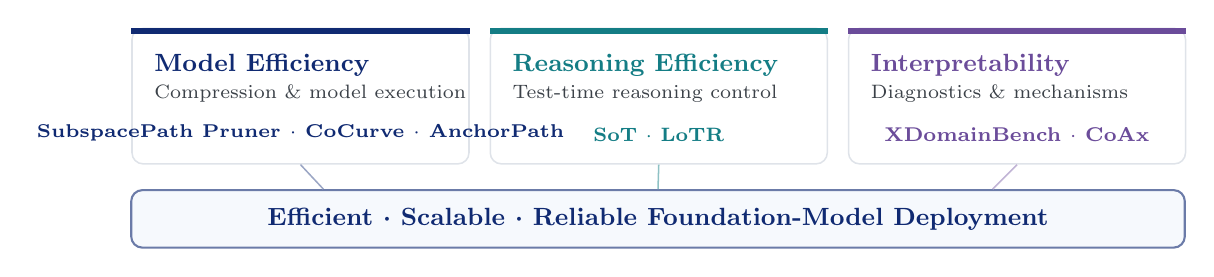
\begin{tikzpicture}[font=\sffamily,x=1cm,y=1cm]
\tikzset{
  domainbox/.style={rounded corners=4pt,draw=MidGray!95,fill=white,line width=.55pt,inner sep=0pt},
  tag/.style={rounded corners=2pt,draw=MidGray!95,fill=SoftGray!80,line width=.32pt,
    inner xsep=3.8pt,inner ysep=2.0pt,font=\scriptsize\bfseries},
  objective/.style={rounded corners=4pt,draw=NTUblue!62,fill=SoftBlue!55,line width=.75pt,
    minimum height=.73cm,align=center,font=\small\bfseries,text=NTUblue}
}
% Three complementary domains. Panels deliberately do not overlap: the diagram shows
% complementarity and contribution to a shared objective, not strict set intersections.
\node[domainbox,minimum width=4.28cm,minimum height=1.72cm,anchor=north west] (d1) at (0,0) {};
\node[domainbox,minimum width=4.28cm,minimum height=1.72cm,anchor=north west] (d2) at (4.55,0) {};
\node[domainbox,minimum width=4.28cm,minimum height=1.72cm,anchor=north west] (d3) at (9.10,0) {};
\fill[NTUblue] (d1.north west) rectangle ([yshift=-.08cm]d1.north east);
\fill[Teal] (d2.north west) rectangle ([yshift=-.08cm]d2.north east);
\fill[Purple] (d3.north west) rectangle ([yshift=-.08cm]d3.north east);

\node[anchor=north west,text=NTUblue,font=\bfseries\small] at ([xshift=.17cm,yshift=-.21cm]d1.north west) {Model Efficiency};
\node[anchor=north west,text=Teal,font=\bfseries\small] at ([xshift=.17cm,yshift=-.21cm]d2.north west) {Reasoning Efficiency};
\node[anchor=north west,text=Purple,font=\bfseries\small] at ([xshift=.17cm,yshift=-.21cm]d3.north west) {Interpretability};

\node[anchor=north west,text=DarkGray,font=\scriptsize] at ([xshift=.17cm,yshift=-.60cm]d1.north west) {Compression \& model execution};
\node[anchor=north west,text=DarkGray,font=\scriptsize] at ([xshift=.17cm,yshift=-.60cm]d2.north west) {Test-time reasoning control};
\node[anchor=north west,text=DarkGray,font=\scriptsize] at ([xshift=.17cm,yshift=-.60cm]d3.north west) {Diagnostics \& mechanisms};

% Project labels: compact text rather than individual chips, to avoid truncation
% while keeping each domain visually readable at report scale.
\node[anchor=south,text=NTUblue,font=\fontsize{6.7}{7.4}\selectfont\bfseries,align=center]
  at ([yshift=.17cm]d1.south) {SubspacePath Pruner $\cdot$ CoCurve $\cdot$ AnchorPath};
\node[anchor=south,text=Teal,font=\scriptsize\bfseries,align=center]
  at ([yshift=.17cm]d2.south) {SoT $\cdot$ LoTR};
\node[anchor=south,text=Purple,font=\fontsize{7.2}{8}\selectfont\bfseries,align=center]
  at ([yshift=.17cm]d3.south) {XDomainBench $\cdot$ CoAx};

\node[objective,minimum width=13.38cm,anchor=north] (obj) at (6.69,-2.05)
  {Efficient $\boldsymbol\cdot$ Scalable $\boldsymbol\cdot$ Reliable Foundation-Model Deployment};
\draw[NTUblue!42,line width=.55pt] (d1.south) -- ([xshift=-4.25cm]obj.north);
\draw[Teal!48,line width=.55pt] (d2.south) -- (obj.north);
\draw[Purple!42,line width=.55pt] (d3.south) -- ([xshift=4.25cm]obj.north);
\end{tikzpicture}
}
\end{center}
\vspace{-1.0mm}

\begin{thesisbox}
\textbf{Core question.} How can foundation models realize \textbf{efficient, scalable, and reliable deployment} under heterogeneous real-world demands, and how can their internal behavior and mechanisms be used to guide adaptation?
\end{thesisbox}

\textbf{Research framework.} The PhD addresses this question at two control levels. \textbf{Part I -- Adaptive Model Execution} adapts the structural capacity exposed by the backbone to the current deployment condition. \textbf{Part II -- Adaptive Reasoning} adapts evidence use, stopping, and internal execution to the current reasoning state. Two background studies motivate the framework: \XDB{}\worktag{D1} shows externally that strong models can still fail when familiar knowledge must be composed under heterogeneous demand, while \CoAx{}\worktag{D2} shows internally that interventions can trigger structured compensation and self-repair. Together they suggest that deployment should exploit, rather than ignore, the structure revealed by model behavior and internals.

{\large\bfseries\color{NTUblue}Part I --- Adaptive Model Execution}\\[-0.7mm]
\begin{itemize}
\item \SubspacePath{}\worktag{E1} -- \textbf{scenario $\rightarrow$ pathway.} Semantic domain axes, layer-wise probes, and cached representation--head coupling compile a reusable scenario-specific attention-head subnetwork without scenario-specific training. The key result is strongest under distribution shift, where one global ranking is least appropriate.
\item \CoCurve{}\worktag{E2} -- \textbf{nodes $\rightarrow$ interactions.} A label-free output-KL risk yields one second-order matrix whose diagonal is node saliency and off-diagonal is co-pruning interaction. A Fisher/Gram identity estimates the matrix from one single-unit ablation per removable unit, after which attention and FFN units share one interaction-aware physical budget. The same formulation transfers from LLMs to VLMs.
\item \AnchorPath{}\worktag{E3} -- \textbf{one shot $\rightarrow$ continuation.} At aggressive sparsity, a dense-point surrogate becomes stale as earlier removals move the operating point. Anchored continuation refreshes the local decision along a nested pruning path, with its largest gains in the high-sparsity regime.
\end{itemize}

\begin{thesisbox}
\textbf{Part-I progression.} Deployment context changes which computation is useful; interactions change the damage of removing a set; aggressive sparsity changes the operating point from which that damage is estimated.
\end{thesisbox}

\newpage

\begin{minipage}[c]{0.78\textwidth}
{\Large\bfseries\color{NTUblue} Executive Summary \textnormal{(continued)}}\\[-1mm]
{\small\color{DarkGray}Towards Efficient, Scalable, and Reliable Foundation Model Deployment}
\end{minipage}\hfill
\begin{minipage}[c]{0.18\textwidth}
\raggedleft
\includegraphics[width=\linewidth]{figures/ntu_logo.png}
\end{minipage}
\vspace{0.5mm}\hrule\vspace{1.1mm}

{\large\bfseries\color{NTUblue}Part II --- Adaptive Reasoning}\\[-0.7mm]
\textbf{Why the control problem continues after deployment.} Even after an efficient model has been selected, different questions---and different steps within the same question---need different evidence, depth, and computation. \XDB{} makes this demand visible at the behavioral level; Part II asks whether the model's own state can become the controller.

\begin{itemize}
\item \SoT{}\worktag{R1} -- \textbf{external script $\rightarrow$ endogenous trajectory control.} A compact state $m_t=[\delta_t,v_t,c_t,H_t]$ summarizes within-step dispersion, progress, directional consistency, and predictive uncertainty. The state controls both which historical evidence remains active and whether reasoning should continue. Across 4 models and 20 datasets, the paper reports improved task quality while reducing generated tokens by \textbf{69.0\%} and latency by \textbf{48.7\%} relative to the compared baselines in aggregate.
\item \LoTR{}\worktag{R2} -- \textbf{logic state $\rightarrow$ internal pathway.} Recurring logic states are learned offline and coupled to reusable attention-head templates. Layer-wise probes infer the current state mixture and compose a step-specific pathway while leaving the outer reasoning paradigm unchanged. Across 3 backbones, 8 benchmarks, and 8 paradigms, the paper reports a \textbf{7.93\% relative average accuracy gain} with \textbf{+3.18\% generated tokens}; realized latency is backbone-dependent, decreasing on Llama and Mixtral while increasing on Qwen.
\end{itemize}

\begin{center}
\resizebox{0.94\textwidth}{!}{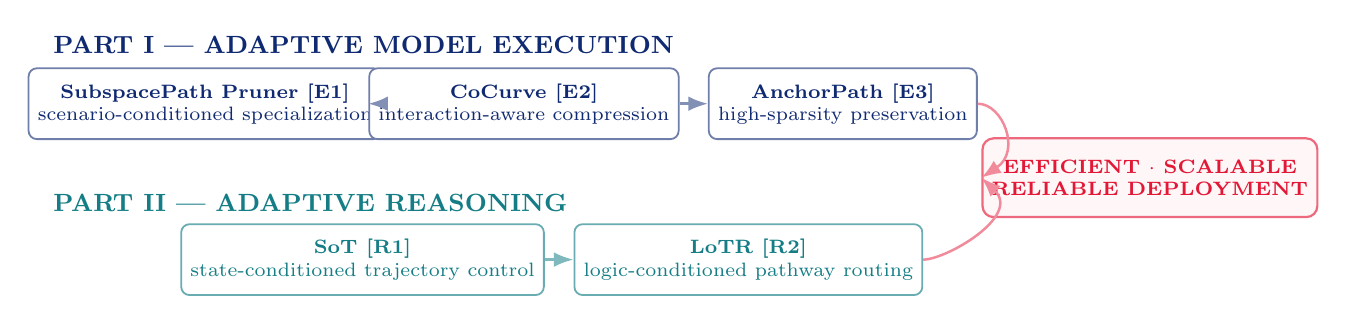
\begin{tikzpicture}[x=1cm,y=1cm,font=\sffamily,>=Latex]
  \tikzset{
    work/.style={rounded corners=3pt,minimum width=3.05cm,minimum height=.90cm,
      align=center,line width=.65pt,font=\bfseries\scriptsize,fill=white},
    goal/.style={rounded corners=4pt,minimum width=3.45cm,minimum height=1.00cm,
      align=center,line width=.8pt,font=\bfseries\scriptsize,fill=NTUred!4,text=NTUred,draw=NTUred!65}
  }
  \node[font=\bfseries\small,text=NTUblue,anchor=west] at (0,1.62) {PART I --- ADAPTIVE MODEL EXECUTION};
  \node[work,draw=NTUblue!60,text=NTUblue] (sp) at (2.05,.88)
    {SubspacePath Pruner [E1]\\\normalfont scenario-conditioned specialization};
  \node[work,draw=NTUblue!60,text=NTUblue] (cc) at (6.10,.88)
    {CoCurve [E2]\\\normalfont interaction-aware compression};
  \node[work,draw=NTUblue!60,text=NTUblue] (ap) at (10.15,.88)
    {AnchorPath [E3]\\\normalfont high-sparsity preservation};
  \draw[->,NTUblue!52,line width=.9pt] (sp.east) -- (cc.west);
  \draw[->,NTUblue!52,line width=.9pt] (cc.east) -- (ap.west);

  \node[font=\bfseries\small,text=Teal,anchor=west] at (0,-.38) {PART II --- ADAPTIVE REASONING};
  \node[work,draw=Teal!64,text=Teal] (sot) at (4.05,-1.10)
    {SoT [R1]\\\normalfont state-conditioned trajectory control};
  \node[work,draw=Teal!64,text=Teal] (lotr) at (8.95,-1.10)
    {LoTR [R2]\\\normalfont logic-conditioned pathway routing};
  \draw[->,Teal!54,line width=.9pt] (sot.east) -- (lotr.west);

  \node[goal] (goal) at (14.05,-.06)
    {EFFICIENT $\cdot$ SCALABLE\\RELIABLE DEPLOYMENT};
  \draw[->,NTUred!50,line width=.9pt] (ap.east) .. controls (12.18,.88) and (12.42,.28) .. (goal.west);
  \draw[->,NTUred!50,line width=.9pt] (lotr.east) .. controls (11.46,-1.10) and (12.42,-.55) .. (goal.west);
\end{tikzpicture}
}
\end{center}
\vspace{-1.3mm}

\begin{smallbox}[What the projects jointly establish]
\begin{tabularx}{\linewidth}{@{}p{2.75cm} X@{}}
\textbf{Conditionality} & Scenario, pruning operating point, reasoning state, logic state, and intervention can all change which computation is useful.\\
\textbf{Relational structure} & Unit damage and causal importance depend on what else is active or removed; evidence and pathway utility depend on the evolving reasoning state.\\
\textbf{Two timescales} & Model execution adapts at deployment/model scale; reasoning adapts at test-time/step scale. The two meet when model-derived state directly controls internal pathways.\\
\end{tabularx}
\end{smallbox}

\begin{thesisbox}
\textbf{Research thesis.} Efficient, scalable, and reliable deployment requires adaptation at two levels: the backbone should expose capacity that matches the current scenario, and the reasoning process should spend effort that matches the current state. Behavioral and mechanistic evidence provides the basis for deciding when that adaptation is justified.
\end{thesisbox}

{\large\bfseries\color{NTUblue}Next-stage research}\\[-0.7mm]
\begin{itemize}
\item \textbf{Deepen adaptive execution and reasoning.} Develop methods with stronger cross-model/domain generalization, explicit uncertainty and fallback behavior, and realized efficiency measured by wall-clock latency, memory, tokens, and physically executed structure.
\item \textbf{Extend to frontier deployment settings.} Study agents and long-horizon systems where tools, retrieval, memory, planning, state drift, delayed feedback, and multimodal/physical-world observations turn adaptive allocation into a system-level problem.
\end{itemize}

\vfill
\footnotesize\color{DarkGray}
\textbf{Project index:} D1 \XDB; D2 \CoAx; E1 \SubspacePath; E2 \CoCurve; E3 \AnchorPath; R1 \SoT; R2 \LoTR.\\[-0.3mm]
\textbf{Website:} \href{https://gongzhiren.github.io/personal-website/}{gongzhiren.github.io/personal-website/}

\end{document}
